\begin{frame}{}
    \LARGE GANs: \textbf{Definition and Core Components}
\end{frame}

\begin{frame}{Definition and Core Components}
\begin{itemize}
    \item Let $S_1 = D = \{x \sim p_{\text{data}}\}$ and $S_2 = \{x \sim p_\theta\}$.
    \item \textbf{Idea}: Train the generative model to minimize a two-sample test objective between $S_1$ and $S_2$, i.e., the generator.
    \item<2-> \textbf{Question}: How do we obtain a two-sample test objective?
    \item<3-> \textbf{Another Idea}: Train another neural network to discriminate between the two samples, i.e., the discriminator.
    \item<4-> And Voila! That's how we arrive at a GAN. The remaining step is to define the training method.
\end{itemize}
\end{frame}

\begin{frame}[allowframebreaks]{GANs: Definition and Core Components}
\begin{figure}
    \centering
    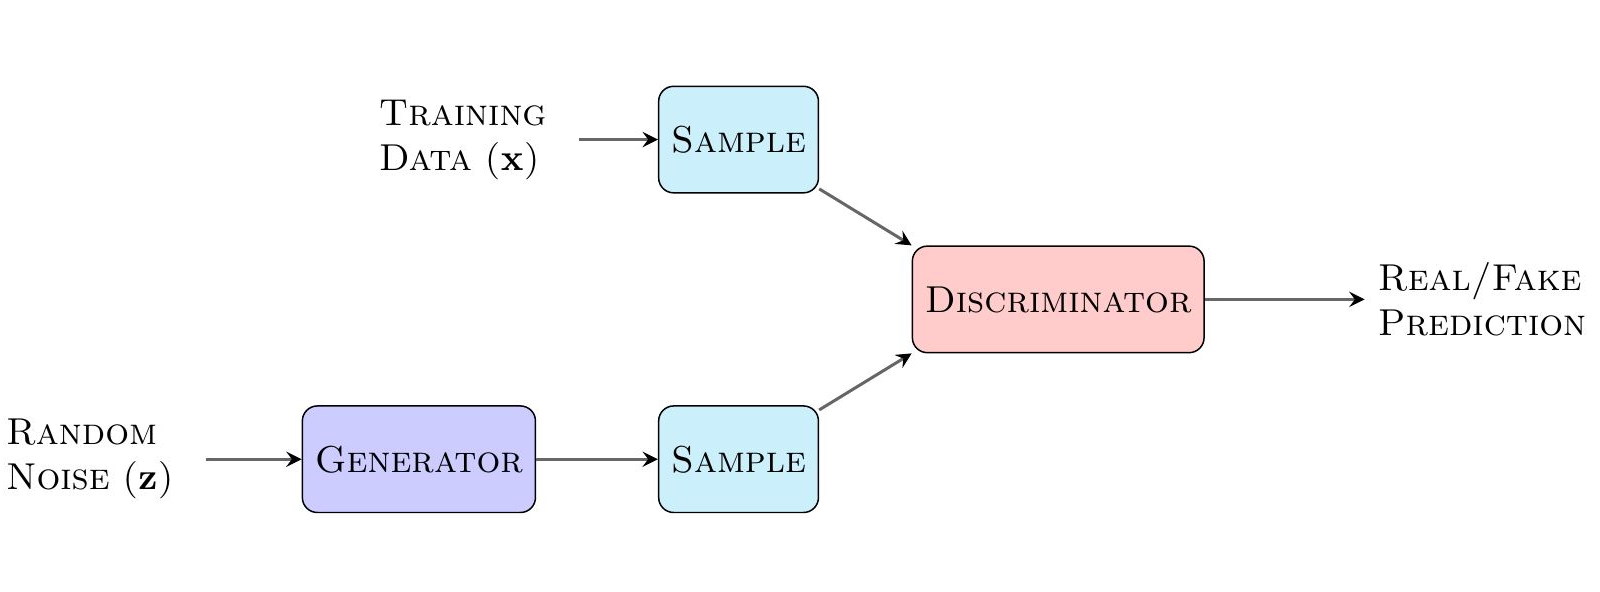
\includegraphics[height=0.7\textheight, width=\textwidth, keepaspectratio]{images/gan/gan_1.png}
    \caption*{A GAN model diagram\footnote{https://github.com/JamesAllingham/LaTeX-TikZ-Diagrams}}
\end{figure}

\framebreak

\begin{itemize}
    \item Generative Adversarial Networks were introduced by Ian Goodfellow et al. (2014).
    \item The idea behind GANs is to train two networks jointly:
    \begin{itemize}
        \item A \textbf{discriminator (D)} to classify samples as “real” or “fake”.
        \item A \textbf{generator (G)} to map a simple fixed distribution to samples that fool \textbf{D}.
    \end{itemize}
    \item The approach is \textbf{adversarial} since the two networks have opposing objectives.
\end{itemize}

\framebreak
\begin{figure}
    \centering
    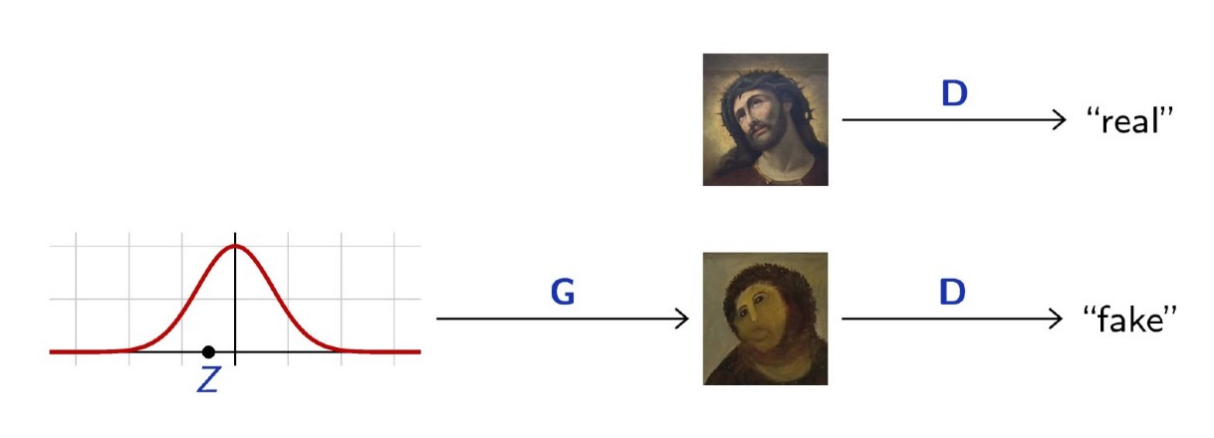
\includegraphics[height=0.7\textheight, width=\textwidth, keepaspectratio]{images/gan/gan_2.png}
    \caption*{The generator transforms a simple distribution into samples resembling real data. The discriminator distinguishes between real and fake samples.}
\end{figure}
\end{frame}